\section{Image Transform}

\subsection{The discrete cosine transform matrix}

\subsubsection{What does each row of the DCT transform matrix represent? Look at the pattern for each row. If you still don't see it, try plotting each of the rows as a 1-D function.}
Each row of the DCT matrix is a cosine wave, with the period equal to $\frac{\pi}{n} \cdot (i-1)$; where $n$ is the number or rows in the DCT and $i$ is the row of the matrix being examined, with the exception of the first row is constant. The transform of the matrix is given by a product of a cosine oscilating in each direction.

\begin{table}[tbhc]
	\caption{Discrete Cosine Transform Matrix}
	\label{tbl:dctm}
	\begin{center}
		\begin{tabular}{ c | c | c | c | c | c | c | c}
0.3536	&	0.3536	&	0.3536	&	0.3536	&	0.3536	&	0.3536	&	0.3536	&	0.3536	\\
\hline
0.4904	&	0.4157	&	0.2778	&	0.0975	&	-0.0975	&	-0.2778	&	-0.4157	&	-0.4904	\\
\hline
0.4619	&	0.1913	&	-0.1913	&	-0.4619	&	-0.4619	&	-0.1913	&	0.1913	&	0.4619	\\
\hline
0.4157	&	-0.0975	&	-0.4904	&	-0.2778	&	0.2778	&	0.4904	&	0.0975	&	-0.4157	\\
\hline
0.3536	&	-0.3536	&	-0.3536	&	0.3536	&	0.3536	&	-0.3536	&	-0.3536	&	0.3536	\\
\hline
0.2778	&	-0.4904	&	0.0975	&	0.4157	&	-0.4157	&	-0.0975	&	0.4904	&	-0.2778	\\
\hline
0.1913	&	-0.4619	&	0.4619	&	-0.1913	&	-0.1913	&	0.4619	&	-0.4619	&	0.1913	\\
\hline
0.0975	&	-0.2778	&	0.4157	&	-0.4904	&	0.4904	&	-0.4157	&	0.2778	&	-0.0975	\\
		\end{tabular}
	\end{center}
\end{table}


\begin{figure}[ht]
\centering
	\subfigure[Heat map]{
	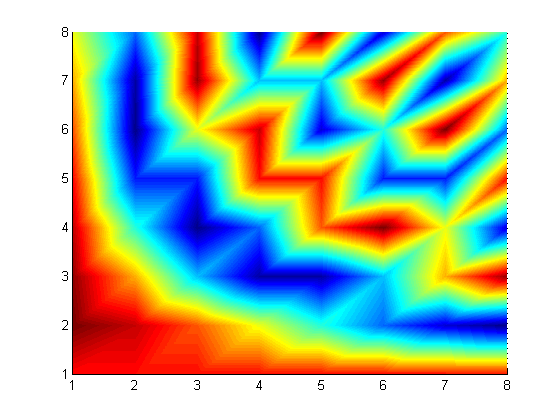
\includegraphics[width=0.45\linewidth]{question3/dctmtx_8_heat}
	}
	\subfigure[Rows of matrix]{
	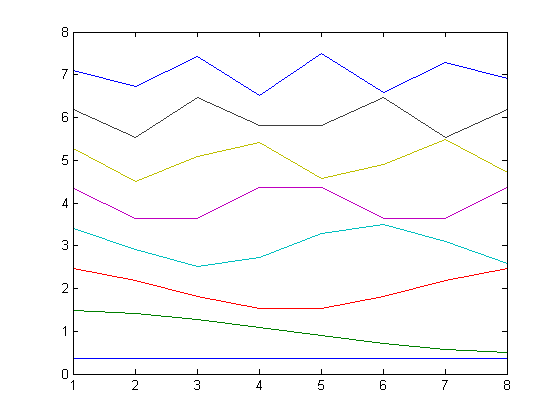
\includegraphics[width=0.45\linewidth]{question3/dctmtx_8_rows}
	}
\end{figure}


\clearpage
\subsection{Applying the discrete cosine transform matrix}


\begin{figure}[ht]
\centering
	\subfigure[Original image]{
	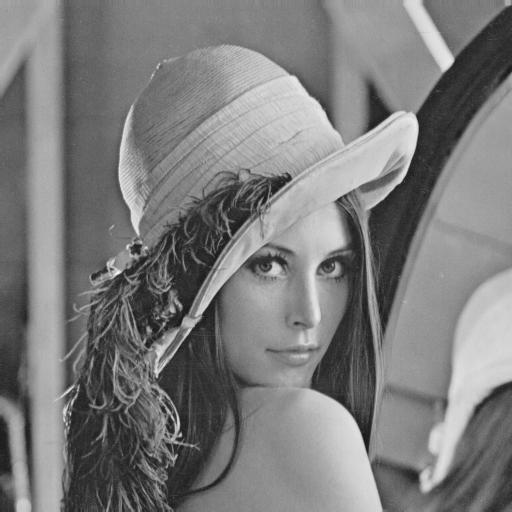
\includegraphics[width=0.45\linewidth]{question3/originalImage}
	}
	\subfigure[DCT 8 $\times$ 8 of original image]{
	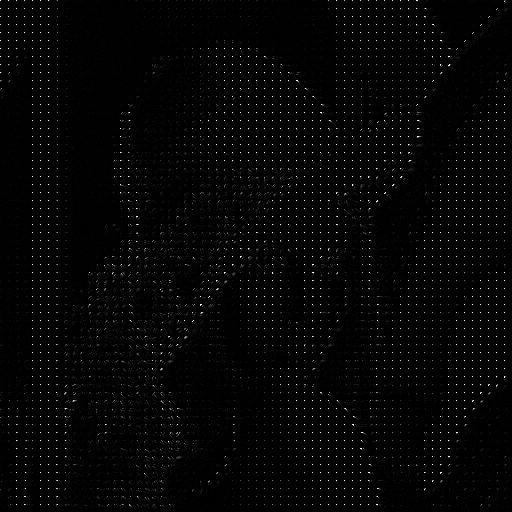
\includegraphics[width=0.45\linewidth]{question3/originalImage_dct}
	}
\end{figure}


\begin{figure}[ht]
\centering
	\subfigure[8 $\times$ 8 image block @ (297,81)]{
	
\includegraphics{question3/block1_8x8}
	}
	\subfigure[DCT]{
		\begin{tabular}{ c c c c c c c c}
		-136 &-31 & 2 &-6 &-1 &-6 &-1 &-4 \\
		14 &-6 & 5 &-6 & 3 &-4 & 2 &-1 \\
		-2 &-3 & 0 &-5 & 3 &-1 & 1 &-2 \\
		1 & 0 & 0 & 2 & 3 &-1 & 0 & 5 \\
		3 & 5 & 0 & 1 & 2 & 4 &-3 & 0 \\
		6 &-1 & 2 & 1 &-1 & 2 & 0 &-1 \\
		0 &-2 & 2 & 0 & 0 &-1 & 0 & 1 \\
		2 &-3 & 0 & 0 &-5 &-3 & 2 & 0 \\
		\\
		\end{tabular}
	}
\end{figure}





	
\begin{figure}[ht]
	\centering

	\subfigure[8 $\times$ 8 image block @ (1,1)]{
	
\includegraphics{question3/block2_8x8}
	}
	\subfigure[DCT]{
		\begin{tabular}{ c c c c c c c c}
		259 & 4 & 3 &-1 & 0 &-1 &-5 & 5 \\
		7 &-1 & 0 &-5 & 1 & 2 &-4 & 3 \\
		-6 &-1 &-2 & 1 &-1 &-1 & 1 &-3 \\
		2 & 1 & 1 & 0 &-1 &-2 & 0 & 1 \\
		-1 &-2 &-1 &-2 & 1 & 1 &-2 &-1 \\
		1 & 0 &-2 &-1 &-3 & 0 & 1 & 0 \\
		-2 & 0 & 3 & 1 & 1 &-3 &-2 &-1 \\
		1 &-1 &-3 &-2 &-1 & 1 & 0 & 0 \\
		\\
		\end{tabular}
	}
\end{figure}


\subsubsection{Describe the energy distribution of the DCT of the sub-images. What does each pixel represent? Explain why DCT would be useful for image compression in the context of the DCT energy distribution}

Most of the energy in the DCT of the images is concetrated in the low frequencies. Each pixel in the DCT represents the intensity of the repsonse of 2D cosine wave of the specified frequency in the original image.

The DCT can be useful in image compression as the ``important'' parts of the image are those that have large values in the DCT. These are low frequncy values. The human perceptual model is also mcuh more sensitive to low frequency detail than high frequency detail, so more lossy compression can be performed in the high frequencies than the low frequencies and still maintain good perceptual quality.

\subsubsection{Compare the DCT of the two sub-images. How are they different? Why? Explain in the context of the image characteristics at those locations and the DCT energy distribution}

The original image block at (1,1) (block 2) is much more uniform than the block at (297,81) (block 1). This corresponds with the DCT for block 2 having most of it's energy restricted to the loweset frequency. Block 1 has slightly more variance in pixel intensities across the block, so the energy distribution of the block is more spread out from the top-left corner.

\clearpage
\subsection{Compressing the DCT image by discarding high-frequency data}

\begin{figure}[ht]
	\centering
	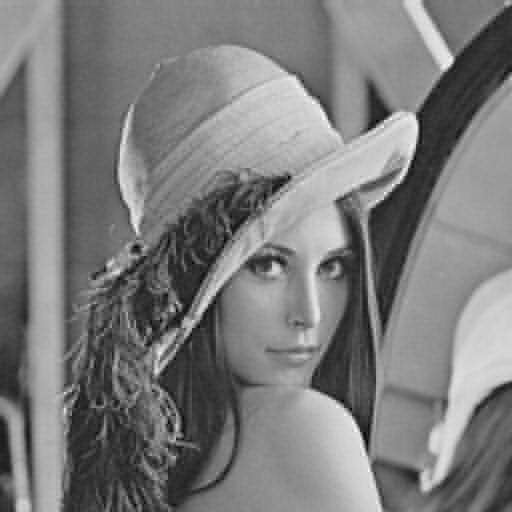
\includegraphics[width=0.55\linewidth]{question3/image_threshold_quant.jpg}
	\caption{Recontstructed image using DCT mask; PSNR +5.80dB}
\end{figure}

\subsubsection{Describe how the reconstructed image looks compared to the original image. Why does it look this way?}

THe reconstructed image looks very similar to the original image, despite it's poor PSNR. The image displays very slight blocking, most visible on the bottom-right most edge of Lena's hat.

These blocking effects occur as all the high frequency data in the image is thrown away, leaving the block to be composed of the DC value, and first and 2nd order cosines. This simplifies the possible gradient that can be displayed in each 8 $\times$ 8 block and can contribute to the appearance of edges around each 8 $\times$ 8 block, contributing to the blocky appearance.


\subsubsection{What artifact is most prominent in the image? Why does this artifact appear?}

The blocking artifact is most prominent in this image. Why this artifact appears is covered in the last paragraph of the previous question.

\subsubsection{What conclusions can you draw about the DCT in terms of image compression? Does it work well? If yes, why does it work well?}

The DCT does not provide a good PSNR from the resulting image, however, the perceptual quality of the image is quite high.

While the pixel intensities my be far from their original values, the structure of the image is maintained by keeping the high energy/low frequency components of the image. This compression method uses 6 values to reprent the DCT matrix which once had 64 values, leading to very good compression, with very litle perceptual loss in quality.